\documentclass[10pt,a4paper]{article}
\usepackage[latin1]{inputenc}
\usepackage{amsmath}
\usepackage{amsfonts}
\usepackage{amssymb}
\usepackage{graphicx}
\author{Jeff Venicx and Jayakrishnan}
\title{Final Project Proposal}
\begin{document}
	
	\maketitle

	\newpage
	
	\section{Introduction}
	for this project we are going to explore methods for classifying music into different sub genres. Using many of the methods that we learned in class including Johnson lindenstraus.
	\section{Distance in song-space}
	
	There are a variety of different methods for calculating a song's distance in song space. The simplest would be using he euclidean distance within the respective dimensions which is the method we are working with as of currently. This is defiantly and area we will explore further to find different distance that will possibly change the effectiveness of our algorithm. 
	
	\section{Dimension reduction and feature extraction}
	
	\subsection{feature extraction}
	The feature vectors of each song help define the distance and similarity measures between the songs to all others. Various spectral and temporal features analysis has to be performed on the tracks to understand how each feature is useful for classification. All the audio features are extracted by taking frames of about 30ms length and computing one feature value for each frame. Some of the features that we intend to analyse are explained below.\\
	\newline
	
	1.	Pitch : Pitch is estimated by performing a series of short term fourier analysis. For each frame the amplitude of the maximum frequency are measured and an approximate greatest common divisor algorithm is used to estimate the pitch.\\
	
	2.	Timbral features: These features describes those characteristics of sound which allow the ear to distinguish tones that have similar loudness and pitch. Every note in the tracks represents a fundamental frequency, but the richness of the music is attributed to the combination of this fundamental along with a series of harmonics. Following are some of the Timbral features.\\
	
	
	2.1.	Zero Crossing rate : It is the average rate at which the song crosses the zero amplitude and it is an excellent feature to distinguish jazz from hard pop. The higher the ZCR, greater the noisiness of the track.
	
	2.2.	Centroid : The spectral centroid is the center of gravity of the spectrum. It gives us an idea of the spectral shape and greater values correspond to brighter textures with more high frequencies. The centroid models the sound sharpness and sharpness is related to the high frequency content of the spectrum.
	
	2.3.	Rolloff:  It's defined as the frequency at which 85 percent of the magnitude distribution of the spectrum is concentrated. Since it has a strong correlation with Centroid and we will choose any one depending on the classification results.
	
	2.4.	Flux:   Flux is an important feature that helps distinguish music from speech and could play a vital role in being a dominant characteristic in genres such as jazz. It is defined as the squared difference between the normalized magnitudes of successive spectral distributions that correspond to successive signal frames.
	
	2.5.	MFCC:  MFCCs try to represent the audio spectrum similar to a human ear's perception making it one of the most powerful features for classifying music. MFCCs can be generated by the following steps. First step is to divide the audio signal into frames of typically 20ms. Next a windowing function is applied to get rid of the edge effects. Then DFT is performed on the frames and take the logarithm f the amplitude spectrum. The resultant spectrum is then converted to a Mel Spectrum.  The Mel Scale is actually a mapping between actual frequency and frequency perceived by the human ear. A human ear doesn't perceive audio in a linear manner. It perceives it as linear below 1 Khz and logarithmic above. The components of the mel spectral vectors are then de-correlated using a DCT.\\
	\newline
	\begin{figure}[h]
		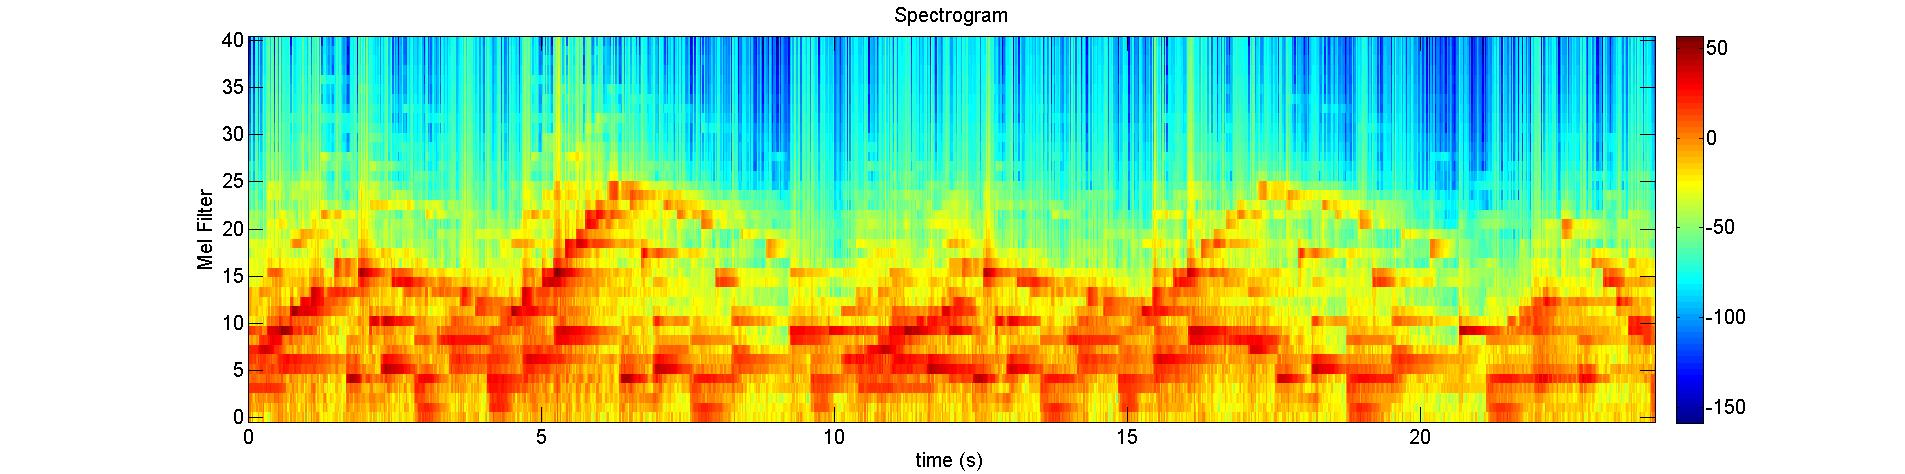
\includegraphics[width = \linewidth]{204_classical}
		\caption{example Mell Spectrum}
	\end{figure}\\
	3.	Rhythmic features: These features bring out structure and regularity  in an audio track. For example the regularity in beats for Electronic or rock is much greater than in Jazz and hence is a very vital feature for genre classification.
	
	3.1.	Beat Strength:  Statistical measures such as mean, standard deviation, derivative mean, third and forth order central moments are evaluated to obtain the overall beat strength of the track.
	
	3.2.	Rhythmic regularity: This can be computed by computing the normalized autocorrelation of the beat histogram. It will contain peaks for rhythmically regular music and a linear plot if it's not rhythmic.
	
	
	\subsection{Dimensionality reduction}
	By performing the aforementioned feature extraction we are already accomplishing significant dimensionality reduction. Further more we started off with random projection to bring down the dimension even further. Using Johnson Lindenstrauss we estimated to what dimension the tracks can be brought down to and then we performed uniform sampling. Some other techniques we want to experiment are
	
	1.	PCA, which performs dimensionality reduction by embedding the data into a linear subspace of lower dimensionality.
	
	2.	ISOMAP, is a technique that addresses issues caused by classical scaling. Classical scaling mainly aims to maintain pairwise Euclidean distance when the datapoints could actually be lying on a curved manifold. ISOMAP addresses this issue by attempting to preserve geodesic distance(curvilinear) between data points.
	
	3.	LLE , constructs a graph representation of the data points. In contrast with other techniques such as ISOMAP or multidimensional scaling, it preserves the local geometric properties.
	
	
	
	
	\section{Statistical Learning}
	We started off performing K nearest neighbors to classify the tracks. It is a relatively simple technique that classifies the songs based on the k nearest songs using a Euclidean distance metric. Some other techniques we wish to experiment with are Neural Networks and Random Forests. Neural networks were chosen for their proven ability to detect complex patterns and model complicated datasets. The random forests algorithm is based on decision trees and unlike neural networks it is robust against over-fitting and it's computationally not expensive.
	
	\newpage
	\section{Initial Results}
	
	For our initial test into classification we reduced the dimensionality of our music set using the MFCC. Then from that data set we used some ideas from Johnson-Lindenstrauss and took random samples from each of the songs to create a space for us to our analysis. We did this in 3 different sized subspaces 20, 100, and 200. Then we used a K-nearest neighbors algorithm with a training set that consisted of 90$\%$ of the given data set and testing with the remaining 10$\%$. then using the sample set we showed the percentage of classifications that were correct. We repeated this process 500 times to get a distribution of how correct the algorithm was able to predict the genres of the sample sets. 
	
	\begin{figure}[htp]
		\centering		
		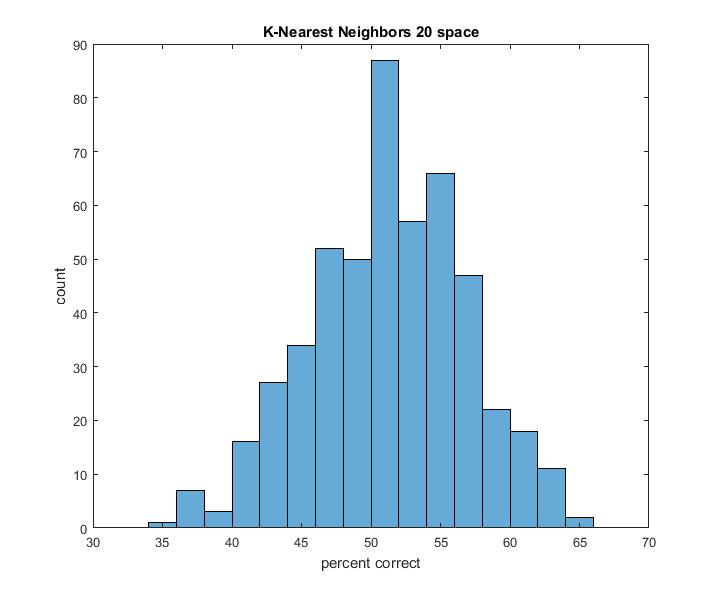
\includegraphics[width = .45\textwidth]{K-Nearest_Neighbor_20.jpg}\quad	
		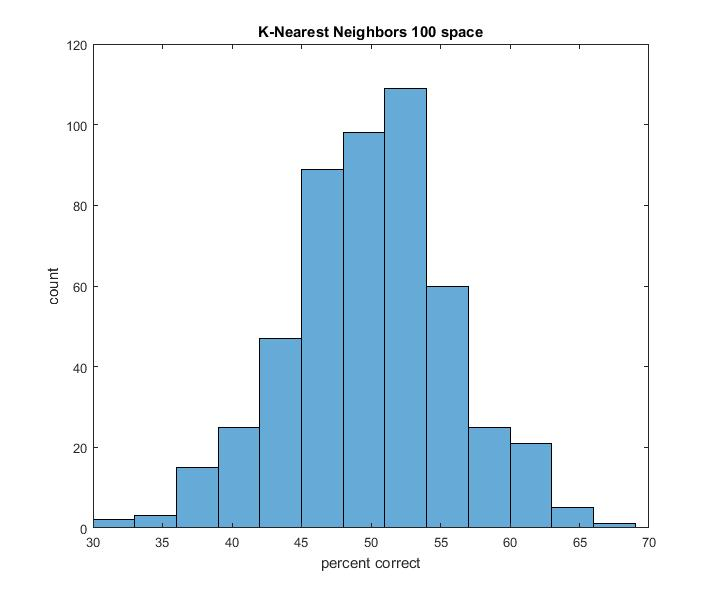
\includegraphics[width = .45\textwidth]{K-Nearest_Neighbor_100.jpg}\quad
		\medskip
		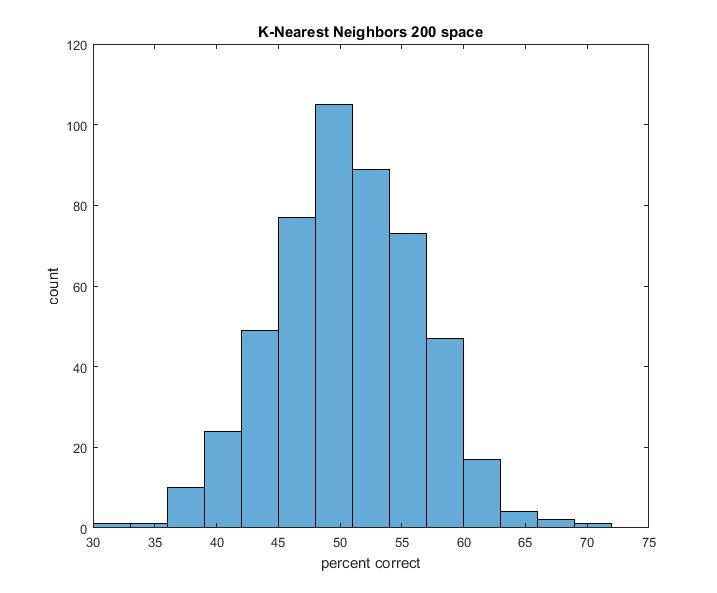
\includegraphics[width = .45\textwidth]{K-Nearest_Neighbor_200.jpg}
	\end{figure}
	with an average of 50$\% $ correct identification its clear that much more advanced statistical methods will be necessary in order to get a more accurate identification.
	
	

	\section{Discussion}
	based on our preliminary results there isn't any one size fits all method for categorizing the data. Our primary path for future research will be to break down which of the dimension reducing methods will allow us to find characteristic features for each genre og music. By using a binary tree to pull out samples that will fall within certain subgroups based on key features we can increase our accuracy as well as decrease the computational time for classification.
	
	Another method involves diving much deeper into the statistical methods that we can use. So far we have not worked with these features and thus will have to make decisions as we explore the different methods.

\end{document}